
\documentclass[a4paper, 11pt]{article}
\usepackage[ascii]{inputenc}
\usepackage{supertabular}
\usepackage[ngerman]{babel}
\usepackage{amsmath}
\usepackage{graphicx}

\usepackage{amssymb,amsfonts,textcomp}
\usepackage {geometry}
\geometry{a4paper,top=25mm,left=30mm,right=25mm,bottom=30mm}
\usepackage{color}
\usepackage{array}
\usepackage{hhline}
\usepackage{hyperref}
\hypersetup{colorlinks=true, linkcolor=blue, citecolor=blue, filecolor=blue, urlcolor=blue}


\begin{document}
{\begin{center}\huge\bf openETCS WP7 Meeting Minutes\end{center}}
\section{Meeting Information}

\renewcommand{\arraystretch}{1.5}
\begin{supertabular}{m{.2\textwidth}m{.8\textwidth}}
%\hline
Subject & WP7 Weekly Scrum: Toolchain\\
Date \& time & 2014-04-25, 11:00h--11:15h\\
Location & Telco and Goto-Meeting\\
%Called up by & Marielle Petit-Doche\\
Called up by & Michael Jastram\\
Participants &
%Mathilde Arnaud,
Benjamin Beichler
Marc Behrens,
Cecile Braunstein,
Fausto Cocchetti,
%Peyman Farhangi,
%Lukasz Fronc,
%Frank Golatowski,
Klaus R\"udiger Hase,
Bernd Hekele,
%Jonas Helming,
%Hardi Hungar,
Baseliyos Jacob,
Michael Jastram,
Peter Mahlmann,
%Huu-Nghia Nguyen,
%Alexander Nitsch,
%Matthieu Perin,
%Marielle Petit-Doche,
%Stan Pinte,
%Ralf Pinger,
%Christophe Ponsard,
%Alexander Stante,
Stefan Rieger,
Uwe Steinke,
%Izaskun de la Torre,
%Giovanni Trotta,
%Jan Welte,
%Jan Welvaarts,
%Giovanni Zanelli,
%Silvano dal Zilio
\\

Minutes by & Bernd Hekele\\

%\hline
\end{supertabular}
\renewcommand{\arraystretch}{1.0}

%\line(1,0){440}

\section{Agenda}
\begin{itemize}
\item Activities
\end{itemize}

\section{Discussion}

\begin{itemize}
\item Activities\\
Michael gave an overview on the resource- situation in the workpackage.
The main drivers for not being able to release more functionality in the toolchain are shown in the following figures.

\begin{figure}
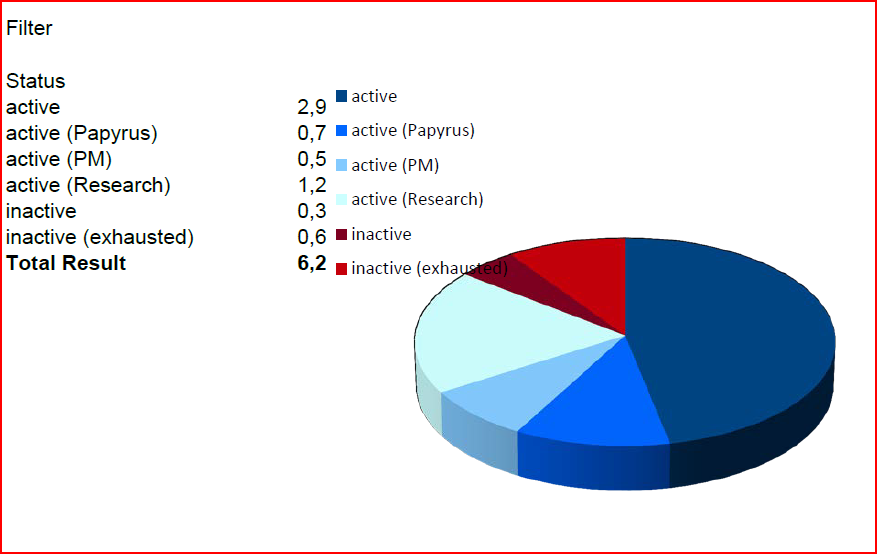
\includegraphics[width=\textwidth]{Figures/Availability.png}
\caption{Availability
\label{f:Availability}}
\end{figure}

\begin{figure}
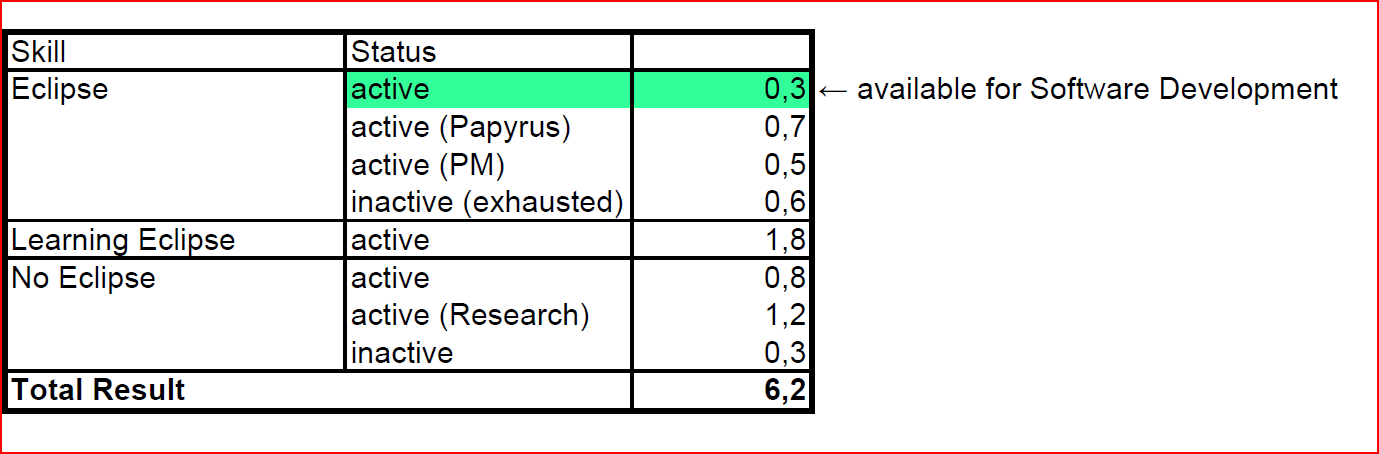
\includegraphics[width=\textwidth]{Figures/Skills.png}
\caption{Skills
\label{f:Availability}}
\end{figure}

\begin{figure}
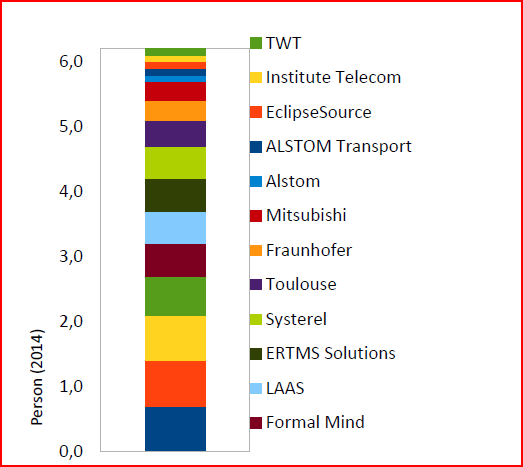
\includegraphics[width=\textwidth]{Figures/Fragmentation.png}
\caption{Fragementation
\label{f:Availability}}

Summary of the situation: to few resources are available and the available resources are strongly fragmented. 

To overcome the situation it was proposed to follow the WP4 example: Implementing strong Agile methods. Details to be discussed in WP7.

\end{figure}

\end{itemize}

\end{document}
